\section{Domain}
\label{sec:domain}
Current automotive in-vehicle networks are mostly based on the Controller Area Network (CAN) and the Local Interconnect Network (LIN) technology for the real-time control of the vehicle. These networks have some drawbacks such as a limited bandwidth which is becoming problematic as functions require more data to be transferred, e.g. autonomous driving. This has led to a redesign of the traditional CAN based function/domain architecture into a zonal architecture where Time Sensitive Networking serves as the main network technology. The remainder of this section explains the main concepts behind CAN in Section~\ref{sec:can}, the challenges and solutions of real-time communication using Ethernet in Section~\ref{sec:real-time-comm} and finally an overview of the domain and zonal architectures is presented in Section~\ref{sec:architectures}.

\subsection{Controller Area Network}
\label{sec:can}
Controller Area Network (CAN) is a networking technology developed by Robert Bosch GMbH in 1983 and later standardized in 1993 as ISO 11898:1993. CAN is an asynchronous serial communication protocol with data rates up to 1 Mbit/s specifically designed for real-time control~\cite{ISO11898} and is organized as a bus architecture. Meaning that each node on the network may transmit a message when it wants, as it is a bus architecture a transmitted message is received by every node on the bus. Carrier Sense Multiple Access/Collision Resolution is used to avoid multiple nodes transmitting concurrently resulting in data errors. The CAN Frame layout together with the physical encoding of the data bits ensures that when two frames are transmitted at the same time the highest priority frame will be delivered. The sender of the lower priority frame detects the collision before data loss occurs and stops transmission, automatically retrying transmission after the higher priority frame is fully delivered. 
\subsection{Real-time communication over Ethernet}
\label{sec:real-time-comm}
Some vehicle functions pose strict timing requirements on the architectures and implementations. For example the passenger safety system must always deploy the airbags within a specific time period after a crash. Deploying the airbags too quickly or too late can cause harm to the passengers. Similarly, when the driver presses the brake pedal in an electric vehicle the car should always stop accelerating, apply regenerative braking and illuminate the brake lights within a well-defined period of time. Large or non-deterministic variations in response time are undesirable from a safety and user experience point of view. Such systems with strict timing requirements are called real-time systems and require the timing properties to be bounded and analysable. 

Traditional automotive networks such as LIN, CAN and FlexRay support real-time communication, while IEEE 802.3 Ethernet is not a real-time network. One of the original design philosophies is best-effort transmission of frames~\cite{metcalfe1976ethernet}. Putting the responsibility of dealing with packet loss, duplication, large delays etc. on the communicating processes. This gives good average-case performance to a large group of users in an economically viable way, but sacrifices the real-time property. The switches used in a full-duplex switched Ethernet network introduce a delay in the communication between two nodes. IEEE 802.3 does not specify how a switch should operate, hence in general no guarantee can be made about the queuing and switching delay added to the transmission time by a switch. Additionally, it is reasonable to assume that queuing delays increase as the number of packets passing through a switch increases. Making Ethernet unsuitable for use in a real-time system. 

Several higher level protocols have been proposed to make real-time communication on top of Ethernet possible e.g EtherCAT, PROFINET, TTEthernet and Time Sensitive Networking. Some of these protocols require special network interface cards or switches to operate, or they are not directly interoperable with standard Ethernet, which complicates mixing the network other devices such as a computer using the TCP/IP stack. Time Sensitive Networking (TSN) is a set of standards created by an IEEE Task Group. According to their website\footnote{\url{https://1.ieee802.org/tsn/}, accessed 15 December 2023} their goal is "\textit{... to provide deterministic connectivity through IEEE 802 networks, i.e., guaranteed packet transport with bounded latency, low packet delay variation and low packet loss.}" TSN standards and amendments can be grouped in four categories according to their design goal~\cite{ashjaei2021time}: Timing and synchronization, resource management, bounded low latency and finally high reliability. For each design goal several solutions have been standardized, e.g. several traffic shapers exist which aim for bounded low latency. Each traffic shaper is designed to solve a different problem, but complicating the network design as many choices need to be made during the design phase. Most standards can be combined in the same network e.g, the Credit Based Shaper~\cite{IEEE8021Qav} and Time Aware Shaper~\cite{IEEE8021Qbv}, increasing design complexity. The relevant standards and amendments for the automotive industry have been summarized in Appendix~\ref{appendix:tsn}.
\subsection{Current and future automotive architecture}
\label{sec:architectures}
Modern vehicles are mostly electrically or electronically controlled, ranging from basic functionality such as accelerating and controlling the lights, to more advanced features such as ride height control through a touch screen or autonomous emergency braking. New European legislation will mandate even more of those functions such as an alcohol interlock, driver drowsiness detection, event data recorders and more. Each function is implemented with one or more dedicated electronic control units (ECUs). The ECUs need to communicate together to achieve a certain function and often need to interface with other functions for data or to achieve a certain safety requirement. The current electrical/electronic control architecture is decentralized, and the networks are grouped based on function. For example a drivetrain network or a body control network. In practice vehicles can have more than 100 ECUs~\cite{bandur2021making} and several communication networks. This has several drawbacks, among others: increased communication load on the network, increased costs, increased software complexity, more software variants, higher maintenance costs and reduced reliability~\cite{bandur2021making}. An example of a decentralized function based architecture can be found in Figure~\ref{fig:functional-arch}, the blue rectangles represent ECUs, ECUs that are part of a single function or domain (body control, drivetrain etc) are connected to each other with an automotive network such as LIN or CAN. The functions or domains work together by means of a gateway (red rectangle) which bridges or translates messages to and from the different networks. Sometimes certain ECUs are also connected to more than one network for practical reasons such as the Steering column ECU in the example.

\begin{figure}[htb]
    \centering
    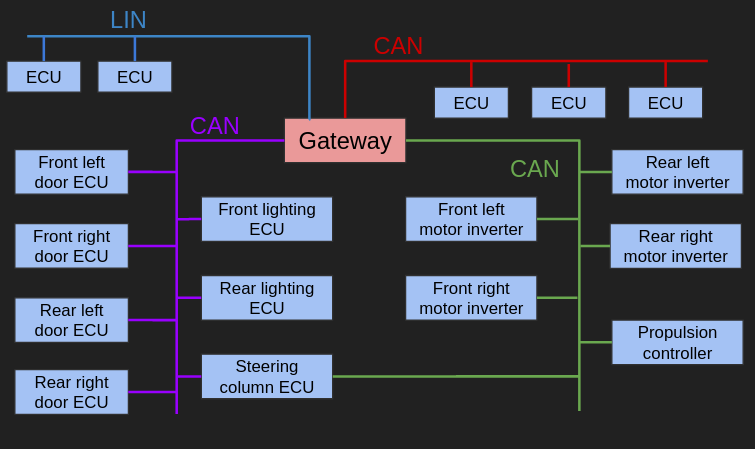
\includegraphics[width=\textwidth]{images/functional-arch.png}
    \caption{Example of an automotive decentralized control architecture}
    \label{fig:functional-arch}
\end{figure}

The rise of advanced driver assistance systems (ADAS) requiring more network bandwidth, extra functions required by European legislation and the aforementioned drawbacks has lead the industry to chose a centralized control architecture with an Ethernet based communication network as the future electrical/electronic architecture, commonly called the zonal architecture~\cite{ashjaei2021time}. Instead of having many small ECUs performing only part of a single function, in the zonal architecture there will be one central ECU responsible for all the control functions and a few larger ECUs, called zone ECUs, which execute the commands of the ECUs. The zone ECUs are strategically placed to handle all functions in the physical neighbourhood of the ECU. To reduce complexity, weight, cost and support ADAS functions, the ECUs are networked through a single high bandwidth, low latency network instead of multiple low bandwidth networks. To ease this transition a zone ECU can act as a bridge for legacy networks used by legacy components in its physical neighbourhood. An example of the zonal architecture with a zone ECU acting as a bridge for a legacy component is shown in Figure~\ref{fig:zonal-arch}

In the new zonal architecture the zone ECU and central controller communicate using a high bandwidth low latency network, automotive Ethernet (single twisted pair physical layer) together with Time Sensitive Networking (TSN) have been chosen as the key networking technologies. The choice for automotive Ethernet is supported by the work of the Time Sensitive Networking (TSN) Task Group of the IEEE 802.1 Working Group, which allow real-time communication over IEEE 802.3 (Ethernet) networks~\cite{klaus2019zonal}. Other relevant factors for choosing automotive Ethernet and TSN are the high bandwidth capabilities relative to traditional networks such as CAN and FlexRay, Internet Protocol (IP) based end-to-end communication support, automotive specific physical layer standards for various data rates, and standardization by the IEEE~\cite{ashjaei2021time}.

\begin{figure}[htb]
    \centering
    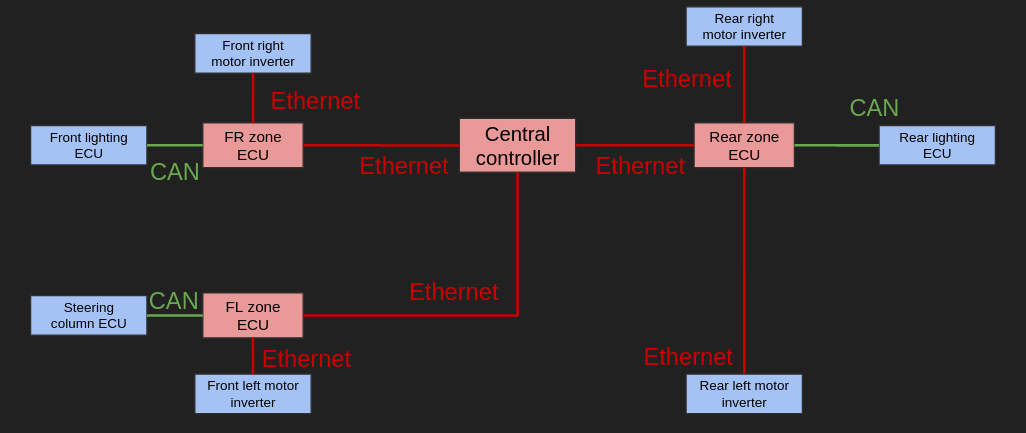
\includegraphics[width=\textwidth]{images/zone-arch.png}
    \caption{Example of an automotive zonal architecture}
    \label{fig:zonal-arch}
\end{figure}

The same vehicle is represented in Figure~\ref{fig:functional-arch} as in Figure~\ref{fig:zonal-arch} but with a decentralized functional architecture and a centralized zonal architecture respectively. The number of ECUs is reduced from 18 to 11 respectively, which is achieved by consolidating ECUs into the zone ECUs, reducing mass. The total number of networks stayed the same, but crucially the physical wiring loom has been simplified in the zonal architecture as there is only a single network going from the back to the front of the vehicle, reducing weight and costs as short wire harnesses can be manufactured automatically.
